\begin{frame}{効くのは日程のずれ：\\1 日で落下点が 43--63 km 動く}{考察}
  \begin{columns}[T]
    \begin{column}{0.58\textwidth}
      {\centering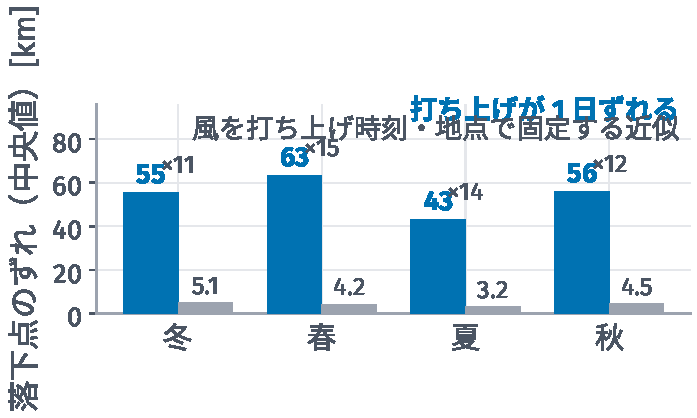
\includegraphics[width=\linewidth,height=100pt,keepaspectratio]{S_slip_vs_frozen.pdf}\par}
      \vskip 0.8mm
      \sub{風を固定する近似の誤差は 3--5 km。\\日程のずれより \kw{1 桁小さく}、直す価値は薄い。}
    \end{column}
    \begin{column}{0.40\textwidth}
      \begin{itemize}\itemsep 1.2mm
        \item \kw{夏}：ずれ 43 km で最小
        \item \kw{秋}：相対誤差 2.9 \% で最小
        \item \warn{春}：ずれ 63 km。避ける
      \end{itemize}
      \vskip 1.5mm
      \sub{すべて「予報が完璧なら」の話。\\予報誤差が上乗せされる。}
    \end{column}
  \end{columns}
  \srcline{北海道、格子の中を実際に飛ばした基準軌道との差（中央値）、2016--2025}
\end{frame}
